\documentclass[12pt, a4paper]{report}
\usepackage[top=3cm,left=3cm,right=2cm,bottom=2cm]{geometry}
\linespread{1.3}
\setlength{\parindent}{1.25cm}
\usepackage{indentfirst}
\usepackage[utf8]{inputenc}
\usepackage[brazil]{babel}
\usepackage{amsmath}
\usepackage{amsthm}
\usepackage{amsfonts}
\usepackage{amssymb}
\usepackage{graphicx}
\usepackage{color}
\usepackage{multicol}
\usepackage[normalem]{ulem}
\usepackage{wrapfig}
\usepackage{caption}
\usepackage{fancybox}
\usepackage[pdfstartview=FitH]{hyperref}
\usepackage{subfigure}
\bibliographystyle{plain}
\usepackage{algorithm}
\usepackage{algpseudocode}
\usepackage{float}


\graphicspath{{Figuras/}}

\renewcommand{\theenumii}{\alph{enumii}}
\DeclareMathOperator{\sen}{sen}
\DeclareMathOperator{\tg}{tg}
\DeclareMathOperator{\arctg}{arctg}
\DeclareMathOperator{\cotg}{cotg}
\DeclareMathOperator{\agm}{agm}

\newtheorem{thm}{Teorema}[section]
\newtheorem{dfn}{Definição}[section]
\newtheorem{prob}{Problema}[section]
\newtheorem{cor}{Corolário}[section]
\newtheorem{prop}{Proposição}[section]
\newtheorem{lem}{Lema} [section]

\newcounter{contar}
%  #endregion preâmbulo

% #region Variáveis 
\newcommand{\nomeUniversidade}{Universidade Federal da Bahia}
\newcommand{\nomeInstituto}{Instituto de Computação}
\newcommand{\nomeCurso}{MATA53 - Teoria dos grafos}
\newcommand{\nomeProfessor}{Islame Felipe da Costa Fernandes}
\newcommand{\nomeGrupo}{\sc{\large{Antoniel Magalhães}} \\
\sc{\large{João Leahy}} \\
\sc{\large{Luis Felipe}}}
\newcommand{\titulo}{\sc{\Large{Problema de Colocação Ótima de Câmeras de Segurança no bairro da Ondina}}}
% #endregion Variáveis 

\begin{document}

% #region capa
\pagestyle{empty}
\begin{center}

\includegraphics[height=2.5cm]{UFBA.jpg}
\hspace{2cm}
\end{center}

\begin{center}
\sc{\large{\nomeUniversidade}} \\
\sc{\large{\nomeInstituto}} \\
\sc{\small{\nomeCurso}} \\

\vspace{4cm}

\titulo

\vspace{4.5cm}

\nomeGrupo


\vspace{5.5cm}

\textbf{Salvador - Bahia} \\
\today
\end{center}
% #endregion capa

% #region folha de rosto
\newpage
\begin{center}
\titulo

\vspace{4cm}

\nomeGrupo
\end{center}

\vspace{4cm}

\begin{flushright}
\begin{minipage}{8.6cm}
Projeto final entregue ao professor \nomeProfessor\ 
como método avaliativo da disciplina \nomeCurso


\end{minipage}
\end{flushright}
 
\vspace{8cm}


\begin{center}
\textbf{Salvador - Bahia} \\
\today
\end{center}

% #endregion folha de rosto

% #region Índice
\newpage
\tableofcontents
\thispagestyle{empty}
\newpage
\setcounter{page}{1}
\pagestyle{plain}
% #endregion Índice


\chapter{Introdução}

\section{Contextualização e Motivação}
A teoria dos grafos oferece um poderoso conjunto de ferramentas matemáticas para modelar e resolver problemas complexos de otimização em redes. No contexto da segurança pública, o problema de posicionamento de câmeras de vigilância pode ser elegantemente modelado como um problema de cobertura mínima de vértices (Minimum Vertex Cover). Nesta abordagem, os vértices do grafo representam possíveis localizações de câmeras, e as arestas representam as áreas que precisam ser monitoradas. O bairro de Ondina, em Salvador, apresenta um cenário ideal para aplicação deste conceito, por concentrar pontos estratégicos como a Universidade Federal da Bahia, estabelecimentos comerciais, hotéis e áreas residenciais, além de um intenso fluxo turístico devido às suas praias.

\section{Justificativa}
A aplicação de conceitos fundamentais da teoria dos grafos, como cobertura de vértices, dominação e problemas de localização de facilidades, fornece uma base teórica sólida para abordar o problema de posicionamento de câmeras. Este trabalho permite explorar na prática diversos algoritmos e técnicas estudados na disciplina MATA53 - Teoria dos Grafos, como algoritmos gulosos, programação dinâmica e métodos de otimização em grafos. A escolha do bairro de Ondina como objeto de estudo possibilita uma aplicação real desses conceitos, contribuindo tanto para o aprendizado acadêmico quanto para uma possível solução prática de segurança pública.

\section{Objetivo Geral e Específicos}
O objetivo geral deste trabalho é aplicar conceitos e algoritmos da teoria dos grafos para desenvolver uma solução que otimize o posicionamento de câmeras de segurança no bairro de Ondina, Salvador.

Os objetivos específicos incluem:
\begin{itemize}
    \item Modelar a região de Ondina como um grafo, onde vértices representam possíveis localizações de câmeras e arestas representam conexões visuais ou físicas entre pontos;
    \item Implementar e comparar diferentes algoritmos estudados na disciplina para resolver o problema de cobertura mínima;
    \item Analisar a complexidade computacional e eficiência dos algoritmos implementados;
    \item Avaliar a aplicabilidade das soluções teóricas em um cenário real de implementação.
\end{itemize}

\section{Metodologia}
\textbf{Modelagem do Problema:} O problema de localização de câmeras de segurança será abordado como um problema de \textbf{cobertura de vértices}, onde:
\begin{itemize}
    \item Os \textbf{vértices} do grafo representam os pontos de interesse a serem monitorados e os potenciais locais de instalação das câmeras.
    \item As \textbf{arestas} representam a visibilidade ou alcance de uma câmera para um determinado ponto de interesse.
\end{itemize}

\textbf{Construção do Grafo:} A região de Ondina será mapeada, identificando pontos estratégicos e possíveis locais de instalação. Um grafo será construído com base nesse mapeamento. Matrizes de adjacência ou listas de adjacência podem ser usadas para representar o grafo.

\textbf{Seleção de Algoritmos:} Serão implementados e comparados algoritmos para resolver o problema de cobertura mínima de vértices. Isso incluirá:
\begin{itemize}
    \item Algoritmos \textbf{heurísticos} para o problema de cobertura de vértices que oferecem soluções aproximadas em tempo polinomial [TODO].
    \item Algoritmos de \textbf{busca em grafos}, como busca em profundidade e largura, que podem ser úteis na identificação de conexões e componentes do grafo [TODO].
    \item  Algoritmos para a determinação de \textbf{conjuntos independentes} [TODO].
\end{itemize}

\textbf{Implementação e Análise:} Os algoritmos serão implementados e testados em instâncias geradas a partir do mapeamento da região de Ondina. A complexidade computacional e a eficiência de cada algoritmo serão analisadas.

\textbf{Avaliação da Aplicabilidade:} A solução obtida será avaliada em um cenário real, considerando a viabilidade prática e a adequação dos resultados.


\section{Organização do Trabalho}
TODO

\section{Trabalhos Correlatos}
O problema de cobertura mínima de vértices tem sido extensivamente estudado na literatura, tanto em sua forma teórica quanto em aplicações práticas. Esta seção apresenta uma revisão dos principais trabalhos relacionados, focando em resultados teóricos fundamentais e aplicações similares ao nosso problema de posicionamento de câmeras.
\subsection*{Conceitos Fundamentais}
\begin{itemize} 
  \item \textbf{Cobertura de Vértices:} Um conjunto de vértices Ĉ de um grafo G é considerado uma cobertura de vértices se toda aresta de G tem pelo menos uma extremidade em Ĉ. O objetivo é encontrar a cobertura de vértices com a menor cardinalidade possível, denotada por b(G) \cite{goldbarg2012}. 
  \item \textbf{Cobertura de Arestas:} Similarmente, um conjunto Ê de arestas é uma cobertura de arestas se todo vértice de G é incidente a pelo menos uma aresta de Ê. A cobertura mínima de arestas é denotada por a(G) \cite{goldbarg2012}. 
  \item \textbf{Complexidade:} Encontrar uma cobertura de arestas em um grafo sem características particulares é um problema polinomial, enquanto encontrar uma cobertura de vértices mínima em um grafo sem características particulares é um problema NP-Difícil \cite{goldbarg2012}. 
\end{itemize}
\subsection*{Resultados Teóricos} 

\begin{itemize} 
  \item A dificuldade de solucionar o problema de cobertura de vértices tem sido objeto de estudo. Dinur e Safra \cite{dinur2005vertexcover} estudam a dificuldade de solução deste problema, enquanto que, se P$\neq$NP, a melhor aproximação possível para esse problema é 1.36 \cite{dinur2005vertexcover}. 
  \item O problema da cobertura conexa mínima admite um fator de aproximação igual a 2 \cite{goldbarg2012}. 
\end{itemize}

\subsection*{Aplicações Similares} 
Vários trabalhos aplicam modelos de localização de facilidades para posicionar recursos de segurança, o que se relaciona com o problema de cobertura de vértices. Por exemplo, no contexto do posicionamento de câmeras de segurança, o objetivo pode ser encontrar um número mínimo de câmeras para cobrir todos os pontos de interesse, ou maximizar a cobertura dada um certo número de câmeras. 
\begin{itemize} 
  \item \textbf{Localização de Câmeras:} O trabalho apresentado em \cite{veloso2021localizacao} busca otimizar a localização de câmeras de segurança em um campus universitário. Nesse contexto, o trabalho aplica variações do Problema de Localização de Facilidades (PLF) e aborda a complexidade do problema devido ao grande tamanho do campus, optando por uma abordagem local. Os modelos aplicados incluem o Problema de Localização com Cobertura Completa (PLCC) e o Problema de Localização com Cobertura Máxima (PLCM), que são usados para determinar o número mínimo de câmeras necessárias para cobrir toda a área e para maximizar a cobertura com um número limitado de câmeras, respectivamente \cite{veloso2021localizacao}. 
  \item \textbf{Outras Aplicações do PLF:} Problemas de localização de facilidades são encontrados em diversas áreas, tais como a localização de sirenes de alertas de tornados, poços de petróleo conectados a plataformas no mar, hubs para transporte aéreo, escolas, e unidades de saúde \cite{veloso2021localizacao}. \end{itemize}

\chapter{Descrição Formal do Problema}

\section{Formalização}
TODO - Definir o problema matematicamente, considerando um grafo \(G = (V, E)\), onde os vértices representam locais possíveis para câmeras e as arestas representam conexões entre pontos.

\section{Restrições do Problema}
TODO - Descrever as restrições, como orçamento limitado, número máximo de câmeras, áreas prioritárias, etc.

\section{Função Objetivo}
TODO - Definir a função que deve ser otimizada, como maximizar a cobertura de áreas críticas ou minimizar o custo total.

\section{Modelagem em Grafos}

A modelagem da malha viária do bairro de Ondina, em Salvador, foi realizada utilizando grafos extraídos do OpenStreetMap. O grafo representa as ruas do bairro, onde os nós correspondem a pontos geográficos (latitude e longitude), e as arestas conectam esses pontos, representando as ruas ou caminhos disponíveis.

\section{Extração, Processamento e Modelagem do Grafo}

A construção do grafo que modela a malha viária do bairro de Ondina em Salvador foi realizada a partir de dados extraídos do OpenStreetMap (OSM). Este processo envolveu múltiplas etapas, desde a coleta dos dados geográficos até a simplificação e ajuste do grafo para adequação ao problema em análise.

\subsection{Extração de Dados}

Os dados do OSM, uma base colaborativa que fornece informações detalhadas sobre vias. Passaram por algumas transformações para obtermos apenas as informações necessárias.


A Figura~\ref{fig:ondina_ruas} apresenta a visualização inicial das ruas do bairro de Ondina, com base nos dados brutos extraídos do OSM.

\begin{figure}[H]
    \centering
    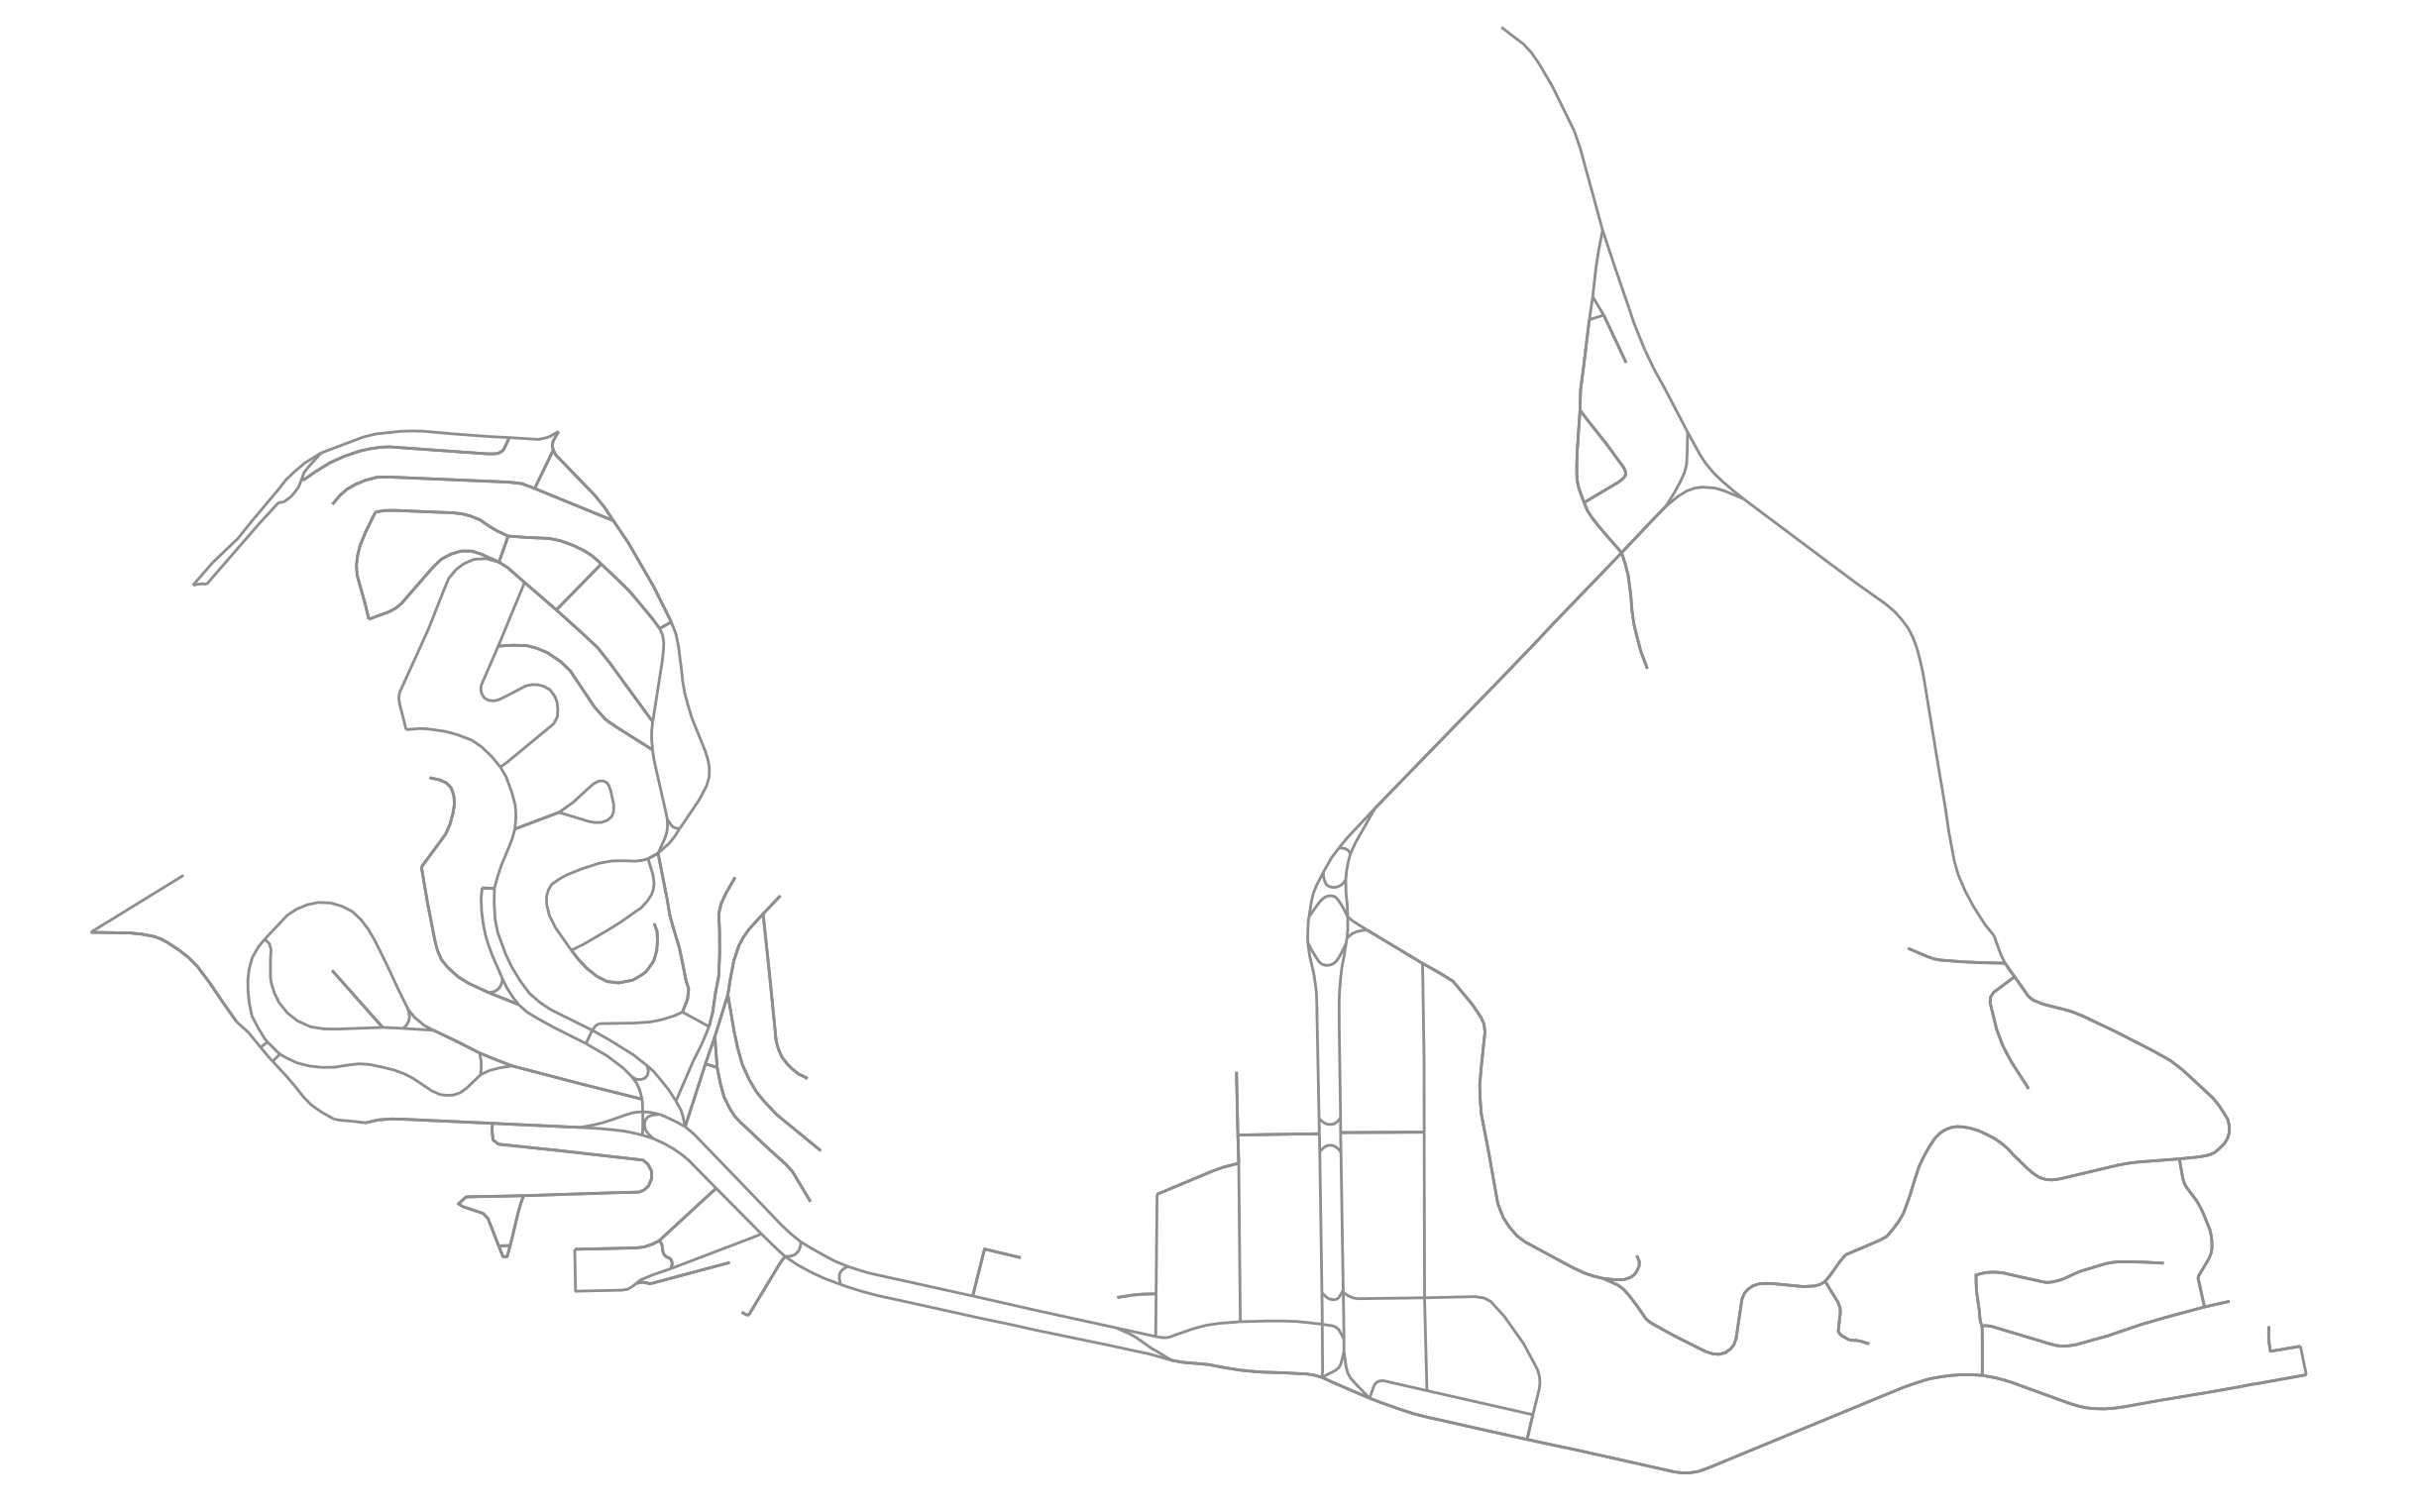
\includegraphics[width=\textwidth]{visualizacao_inicial}
    \caption{Visualização inicial das ruas do bairro de Ondina.}
    \label{fig:ondina_ruas}
\end{figure}

\subsection{Processamento e Construção do Grafo}

Após a extração dos dados, foi realizado o mapeamento para um grafo. Nesta etapa, os nós foram associados aos pontos geográficos, enquanto as arestas representaram as conexões entre eles, sendo atribuído um peso correspondente à distância entre os pontos. A Figura~\ref{fig:ondina_grafo_bruto} mostra a visualização das ruas com os vértices associados.

\begin{figure}[H]
    \centering
    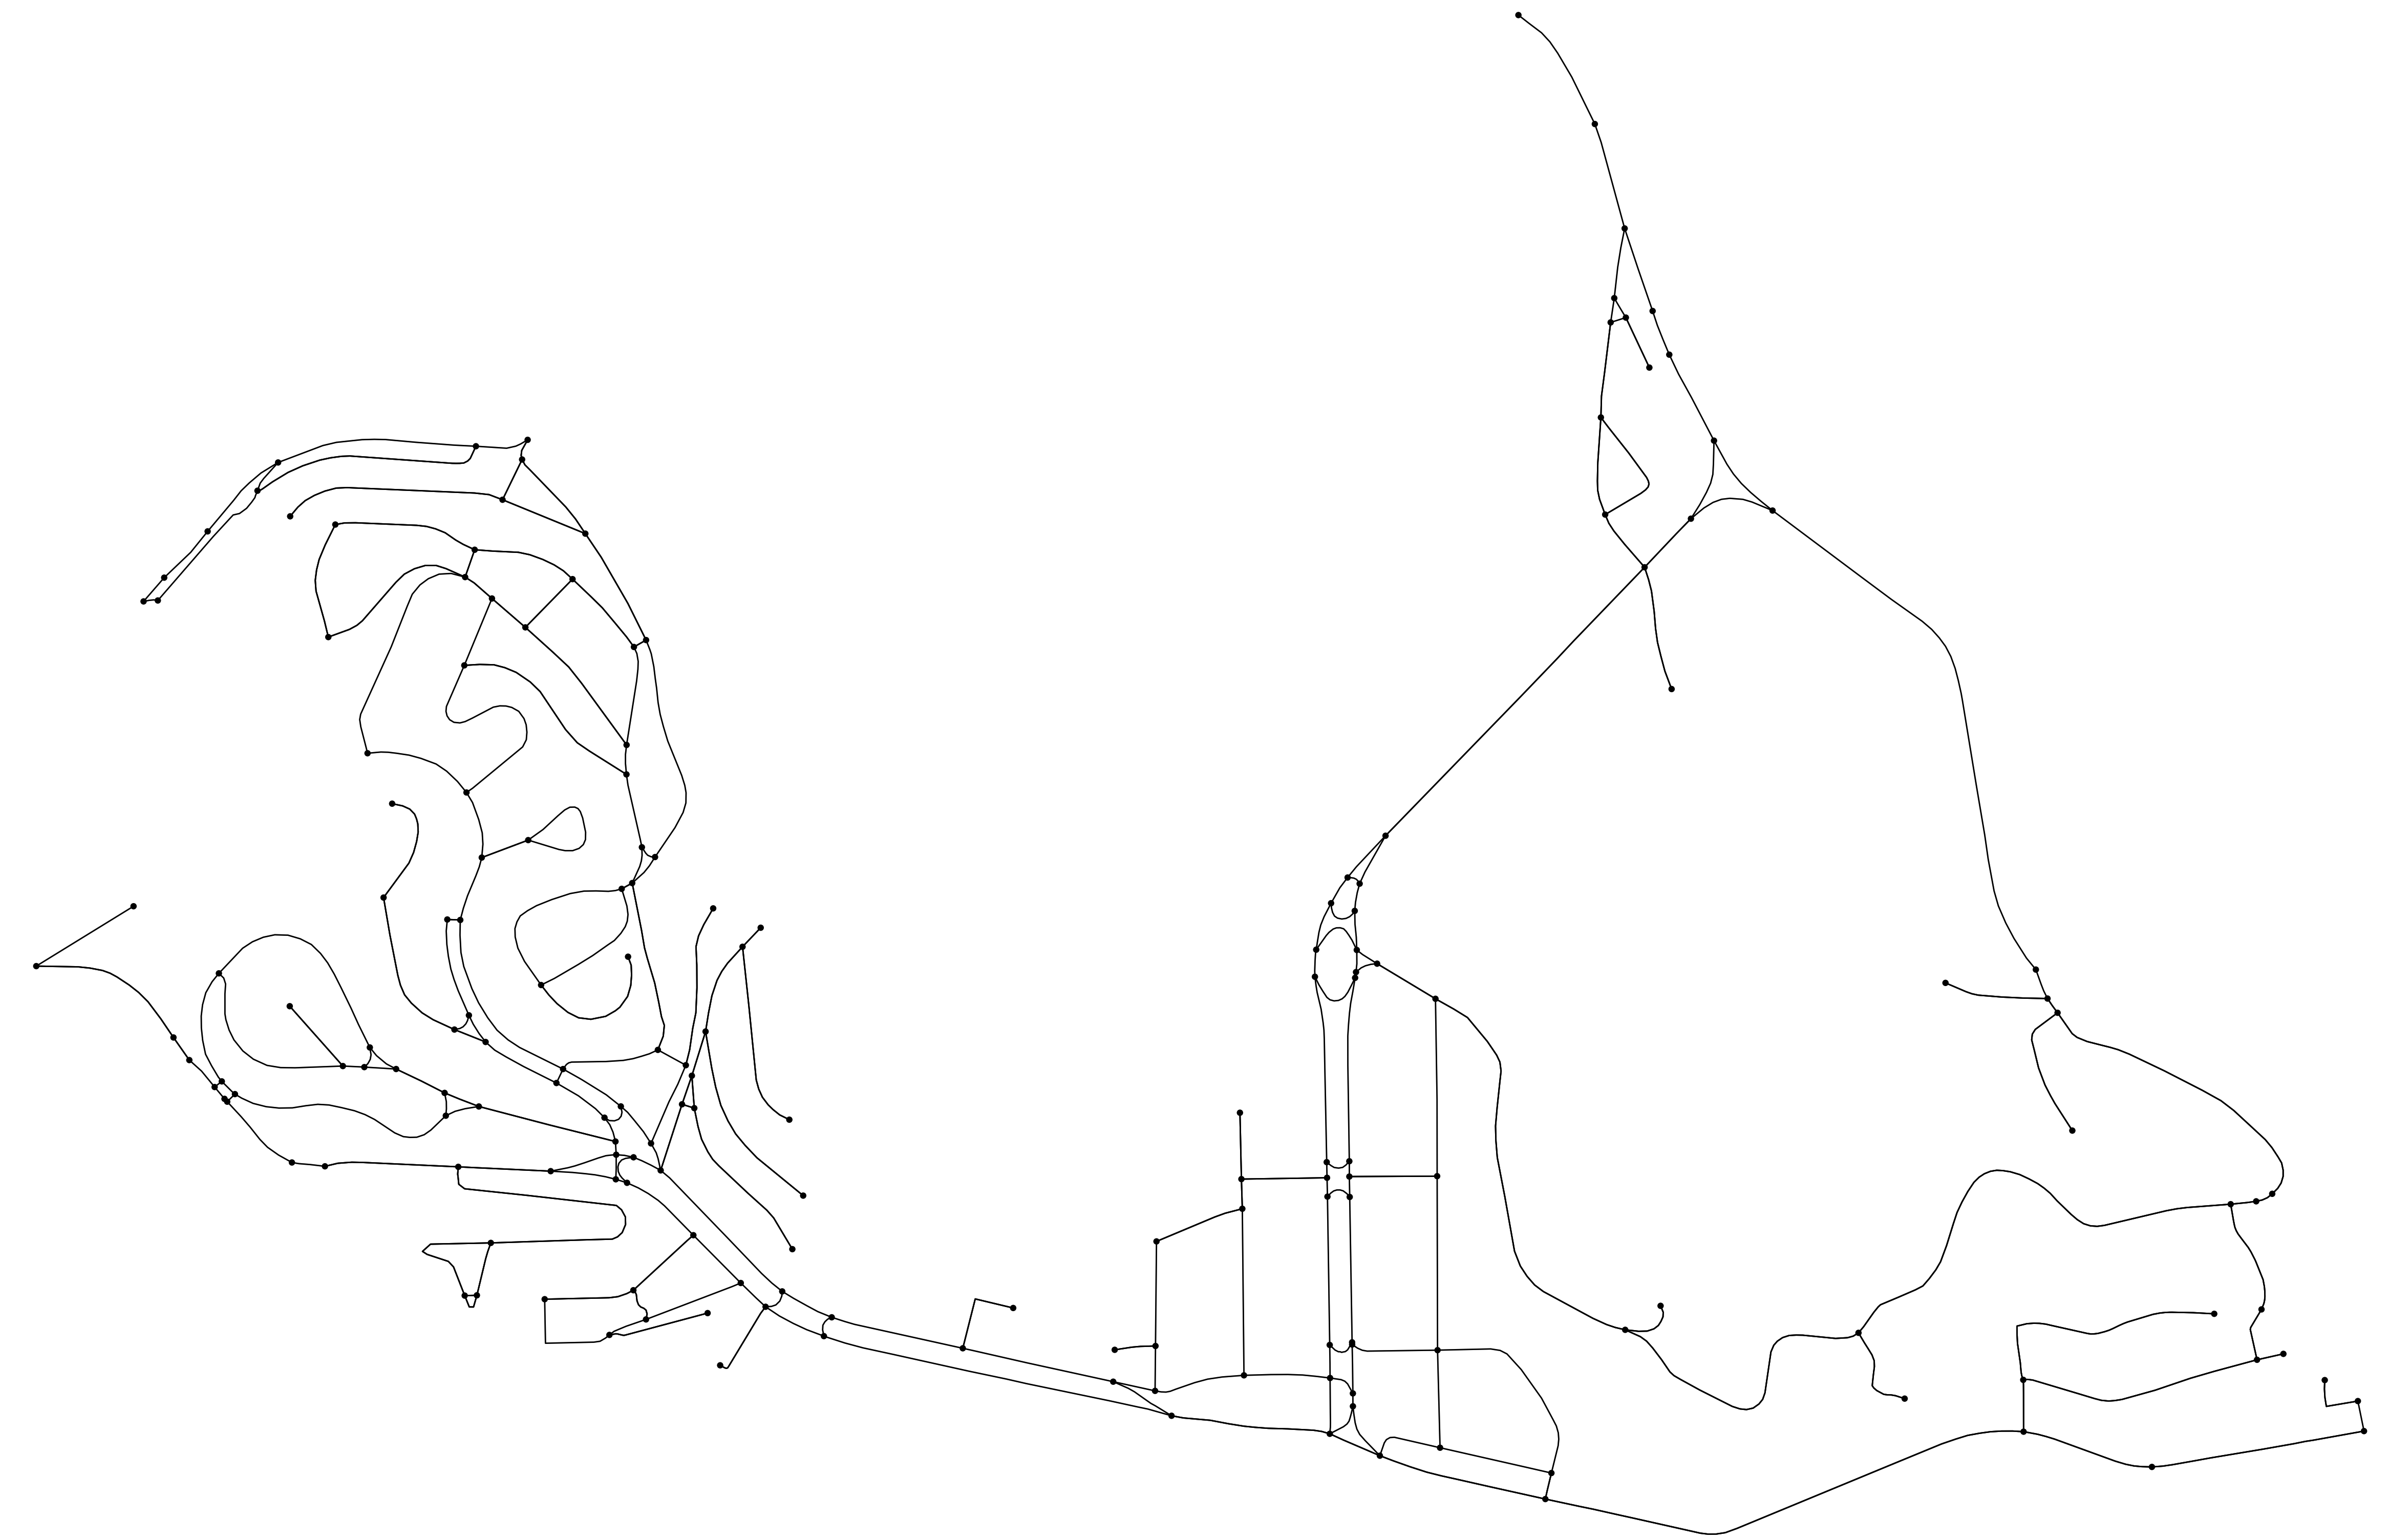
\includegraphics[width=\textwidth]{ondina_grafo_bruto}
    \caption{Visualização das ruas do bairro de Ondina com os vértices associados.}
    \label{fig:ondina_grafo_bruto}
\end{figure}

\subsection{Simplificação do Grafo}

Para adequar o grafo ao problema em análise, foi realizada uma simplificação que assumiu a existência de um campo de visão claro entre os nós conectados por uma aresta. Esta suposição eliminou obstáculos visuais e permitiu modelar de forma idealizada o problema, mantendo apenas os elementos essenciais para a análise.

O resultado do grafo simplificado é apresentado na Figura~\ref{fig:ondina_grafo_simplificado}, mostrando a estrutura final com as simplificações implementadas.

\begin{figure}[H]
    \centering
    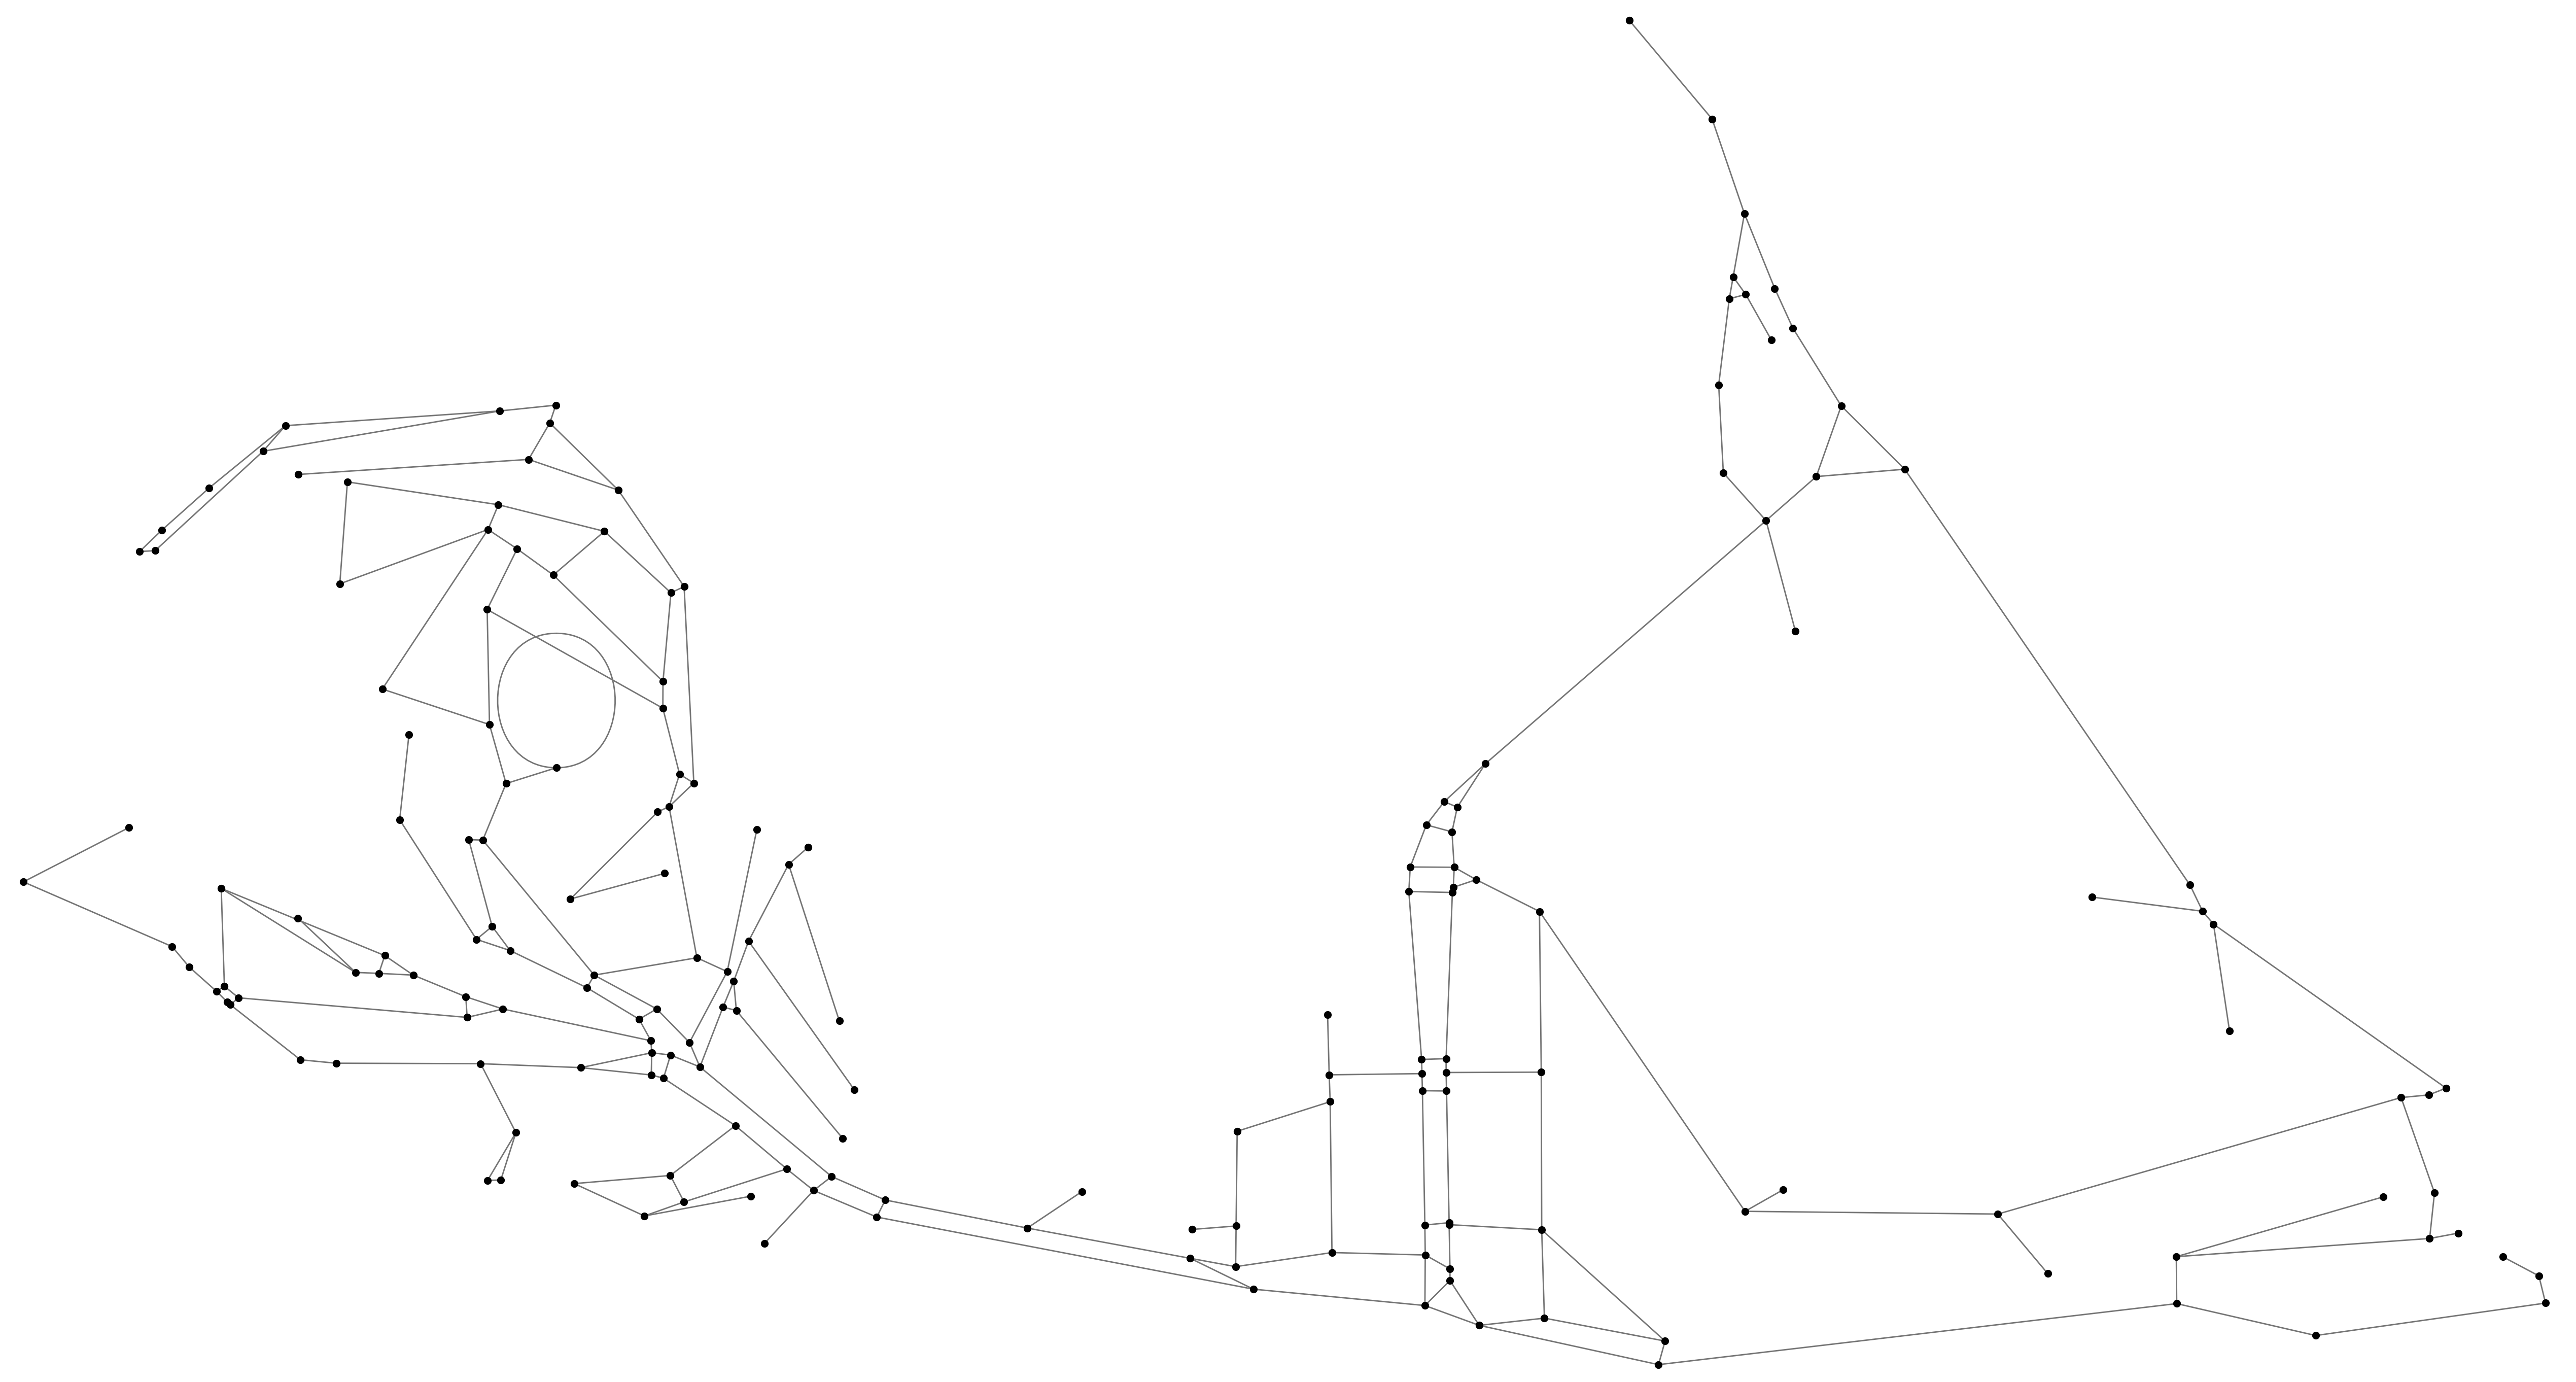
\includegraphics[width=\textwidth]{ondina_grafo_simplificado}
    \caption{Visualização do grafo simplificado do bairro de Ondina.}
    \label{fig:ondina_grafo_simplificado}
\end{figure}

\subsection{Discussão}

A simplificação realizada, ao assumir a existência de campo de visão claro entre os nós, possibilitou o uso do grafo para aplicações práticas no problema em análise. Essa abordagem é particularmente útil em cenários que envolvem monitoramento ou comunicação direta, como a análise de cobertura por câmeras, onde barreiras visuais poderiam ser tratadas como elementos externos ao modelo principal.

O processo de extração, construção e simplificação do grafo demonstra como é possível transformar dados geográficos brutos em representações abstratas otimizadas para resolver problemas específicos. A estrutura final do grafo oferece um modelo compacto e eficiente, adequado para o estudo da cobertura de vértices no contexto urbano de Ondina.
\subsection{Estrutura do Grafo}

O grafo é definido como um conjunto de \textbf{nós} e \textbf{arestas}, organizados da seguinte forma:

\begin{itemize}
    \item \textbf{Nós (Nodes):}
    Cada nó representa um ponto no mapa, definido por suas coordenadas geográficas:
    \begin{itemize}
        \item \texttt{id}: Identificador único do nó.
        \item \texttt{lat}: Latitude do ponto.
        \item \texttt{lon}: Longitude do ponto.
    \end{itemize}
    Exemplo de definição de nós:
\begin{verbatim}
{
  "id": 0,
  "lat": -13.000871,
  "lon": -38.5054976
},
{
  "id": 1,
  "lat": -13.0016275,
  "lon": -38.5057271
}
\end{verbatim}

    \item \textbf{Arestas (Edges):}
    As arestas conectam dois nós, representando ruas ou trechos que ligam os pontos geográficos. Cada aresta é caracterizada por:
    \begin{itemize}
        \item \texttt{source}: Identificador do nó de origem.
        \item \texttt{target}: Identificador do nó de destino.
        \item \texttt{weight}: Peso da aresta, que pode ser interpretado como a distância entre os dois pontos.
        \item \texttt{name}: Nome da rua ou caminho.
    \end{itemize}
    Exemplo de definição de arestas:
\begin{verbatim}
{
  "source": 0,
  "target": 3,
  "weight": 99.5182593770244,
  "name": "Avenida Anita Garibaldi"
},
{
  "source": 1,
  "target": 3,
  "weight": 96.76899596360965,
  "name": "Avenida Milton Santos"
}
\end{verbatim}
    \item \textbf{Metadados:}
    O grafo também inclui informações descritivas adicionais, como:
    \begin{itemize}
        \item \texttt{name}: Nome do grafo, neste caso, "Grafo de Ondina".
        \item \texttt{description}: Descrição geral, como "Grafo das ruas do bairro de Ondina, Salvador".
        \item \texttt{source}: Fonte dos dados, como "OpenStreetMap".
    \end{itemize}
\end{itemize}


\chapter{Solução Algorítmica}

\section{Pseudo-Código}
TODO - Apresentar um algoritmo de alto nível, como um GRASP ou uma abordagem baseada em programação linear.

\section{Detalhes de Implementação}
\subsection{Classes, Diagramas, Estruturas}
TODO - Detalhar a estrutura do código, como organização das classes e métodos.

\chapter{Experimentos}

\section{Metodologia}
\subsection{Instâncias}
TODO - Descrever os dados utilizados, como mapas do bairro da Ondina e pontos potenciais para câmeras.

\subsection{Parâmetros}
TODO - Explicar os parâmetros ajustados nos experimentos, como alcance das câmeras, custo, etc.

\subsection{Testes e Critérios de Análise}
TODO - Detalhar como os resultados serão avaliados (tempo de execução, cobertura alcançada, etc.).

\section{Resultados}
TODO - Apresentar os resultados dos experimentos em gráficos ou tabelas.

\subsection{Avaliação dos Resultado~}
TODO - Analisar os resultados obtidos, comparando as soluções encontradas com os critérios de avaliação.

\chapter{Considerações Finais}

\section{Conclusão}
TODO - Resumir as contribuições e os resultados obtidos.

%-------------Bibliografia------------------
\newpage
\renewcommand{\refname}{Referências Bibliográficas}
\addcontentsline{toc}{chapter}{Referências Bibliográficas}
\bibliography{Bibliografia}
\nocite{*}

\end{document}